% Single source for the LRU comparison report.
% Diagram sources are the filecontents blocks. Rebuild with ./build.sh.
\documentclass[a4paper,11pt,oneside,headings=small,parskip=half,titlepage=false]{scrreprt}

\usepackage[T1]{fontenc}
\usepackage{lmodern}
\usepackage[british]{babel}
\usepackage{csquotes}
\usepackage{microtype}
\usepackage{setspace}
\singlespacing
\usepackage{geometry}
\geometry{a4paper,margin=1in,bindingoffset=0.5in,headheight=16pt}
\usepackage{siunitx}
\sisetup{detect-weight=true,range-phrase=--}
\usepackage{booktabs}
\usepackage{tabularx}
\usepackage{array}
\usepackage{graphicx}
\usepackage{float}
\usepackage{enumitem}
\setlist{itemsep=0.25em,topsep=0.4em}
\usepackage{amsmath}
\usepackage[
  backend=biber,
  style=numeric,
  sorting=none,
  giveninits=true,
  maxbibnames=4,
  doi=true,
  url=true
]{biblatex}
\addbibresource{references.bib}
\usepackage{hyperref}
\hypersetup{hidelinks,pdftitle={Direct-mapped and LRU},pdfauthor={Author name}}
\usepackage{cleveref}

\emergencystretch=2em
\graphicspath{{fig/}}
\setcounter{tocdepth}{2}
\setcounter{secnumdepth}{3}

\begin{filecontents}[overwrite,noheader]{fig/states.mmd}
%%{init: {"theme": "neutral"}}%%
stateDiagram-v2
  [*] --> IDLE
  IDLE --> COMPARE: request
  COMPARE --> RETURN: tag matches a valid line
  COMPARE --> FETCH: miss
  FETCH --> RETURN: four bytes stored
  RETURN --> IDLE: byte returned
\end{filecontents}

\begin{filecontents}[overwrite,noheader]{fig/conflict-dm.json}
{
  "signal": [
    { "name": "request",  "wave": "10.10.10.10." },
    { "name": "miss",     "wave": "01.01.01.01." },
    { "name": "hit",      "wave": "0..........." },
    { "name": "mem_read", "wave": "010.10.10.10" }
  ],
  "head": { "text": "Direct-mapped conflict" }
}
\end{filecontents}

\begin{filecontents}[overwrite,noheader]{fig/conflict-lru.json}
{
  "signal": [
    { "name": "request",  "wave": "10.10.10.10." },
    { "name": "miss",     "wave": "01.01.0....." },
    { "name": "hit",      "wave": "0......10.10" },
    { "name": "mem_read", "wave": "010.10......" }
  ],
  "head": { "text": "LRU conflict" }
}
\end{filecontents}

\begin{filecontents}[overwrite,noheader]{fig/replace-dm.json}
{
  "signal": [
    { "name": "request",  "wave": "10.10.10.10." },
    { "name": "miss",     "wave": "01.0.01.01." },
    { "name": "hit",      "wave": "0...10......" },
    { "name": "mem_read", "wave": "010..10.10.." }
  ],
  "head": { "text": "Direct-mapped replacement" }
}
\end{filecontents}

\begin{filecontents}[overwrite,noheader]{fig/replace-lru.json}
{
  "signal": [
    { "name": "request",  "wave": "10.10.10.10." },
    { "name": "miss",     "wave": "01.0.01.0.." },
    { "name": "hit",      "wave": "0...10...10" },
    { "name": "mem_read", "wave": "010..10...." }
  ],
  "head": { "text": "LRU replacement" }
}
\end{filecontents}

\begin{document}

\titlehead{Computer architecture project report}
\subject{Fully associative LRU, compared with the direct-mapped cache}
\title{Same Capacity, Different Replacement:\\A Fully Associative LRU Cache}
\author{[Author name]\\[0.35em]
\normalsize [Programme], [Institution]\\
\normalsize [Course code]}
\date{10 November 2026}
\publishers{Simulation of the LRU cache. The direct-mapped cache is the board design.}
\maketitle

\begin{abstract}
\noindent
The direct-mapped cache already on the Shrike Lite holds 16~bytes as four lines of four bytes. This report adds a second cache of the same size and asks only what the organisation changes. The second cache is fully associative and replaces the least recently used line. It lives in its own folder and was simulated on its own. The two designs were not placed on the FPGA together.

Both caches see the same read-only memory, in which the byte at an address is the address. A hit returns that byte and leaves memory idle. A miss reads the aligned four-byte line once, stores it, and returns the requested byte. Exhaustive simulation of the LRU cache covered \num{1498} accesses: \num{1076} hits and \num{422} misses. Every miss read memory. No hit did.

Temporal locality and spatial locality produce the same hit and miss sequence on both organisations, because a repeated byte and the other bytes of a freshly filled line are hits either way. The traces separate on conflict and on replacement. Two blocks that share a direct-mapped line can sit together in the associative cache, so the second visit hits. The least recently used rule is checked by leaving one of four resident blocks untouched and confirming that the next new block replaces that one.
\end{abstract}

\noindent\textbf{Keywords:} cache, fully associative, least recently used, direct mapping, conflict miss.

\tableofcontents

\chapter{Why a second cache}
\label{ch:why}

A cache earns its keep when a small store answers references that would otherwise go to a larger memory~\cite{hennessy2017,patterson2021}. The board design already shows that for one organisation: a direct-mapped cache of four lines. Making that cache larger would raise the hit rate for an uninteresting reason. The useful question is what changes when the same sixteen bytes are organised differently.

The second design is therefore the same capacity, four lines of four bytes, and a different placement rule. Any block may occupy any line. When a fifth distinct block arrives, the line that has gone longest without a use is the one overwritten. That is least-recently-used replacement, the policy textbooks set beside direct mapping when they discuss conflict~\cite{hill1989,patterson2021}.

The two caches are not run at the same time. The LRU sources, the testbench and this report are in the folder \texttt{lru/}. The direct-mapped design on the Shrike Lite is unchanged. The comparison in \cref{ch:compare} is the only place the two policies meet, and they meet as two columns of the same short address lists.

\chapter{The two organisations}
\label{ch:org}

Main memory is 256~bytes, addressed by \texttt{address[7:0]}. A read of address \(A\) returns the byte \(A\). Both caches are read-only. A line is the aligned group of four bytes whose address ends in \texttt{00}.

\section{Direct-mapped placement}

The direct-mapped cache uses the address as three fields. The index \texttt{address[3:2]} selects one of the four lines. The tag \texttt{address[7:4]} is compared with the tag stored in that line, and only if the line is valid. The offset \texttt{address[1:0]} selects the byte inside the line. Addresses \texttt{0x00} and \texttt{0x10} share index~0. Installing one of them removes the other, even though three lines are empty. That is a conflict miss: the working set would fit, and the index function still collides~\cite{hill1989}.

\section{Fully associative placement}

The LRU cache has no index. The tag is \texttt{address[7:2]}, six bits, so the tag names the block. The offset is still \texttt{address[1:0]}. A hit is a valid line whose tag equals the requested block. The four lines are searched together.

Each line carries an age in \(\{0,1,2,3\}\). Age~0 is the most recently used line. Age~3 is the least recently used. On a miss the cache prefers an invalid line, the lowest index among the empty ones, and only then the valid line with the greatest age. After a hit or a fill, the touched line becomes age~0 and every other line that was younger than it ages by one. Lines that were already older keep their age. The ages of the four lines stay a permutation of \(0,1,2,3\).

\begin{table}[ht]
\centering
\caption{Ages after filling \texttt{0x00}, \texttt{0x04}, \texttt{0x08} and \texttt{0x0C} into an empty cache, in that order. The first block is the least recently used.}
\label{tab:ages}
\begin{tabular}{lcccc}
\toprule
Line & 0 & 1 & 2 & 3 \\
\midrule
Block & \texttt{0x00} & \texttt{0x04} & \texttt{0x08} & \texttt{0x0C} \\
Age & 3 & 2 & 1 & 0 \\
\bottomrule
\end{tabular}
\end{table}

\section{Hit, miss and the memory read}

The controller has four states, shown in \cref{fig:states}. \texttt{IDLE} waits for a one-cycle request and latches the tag and offset. \texttt{COMPARE} searches the four lines. A hit updates the age and goes to \texttt{RETURN} with memory idle. A miss latches the victim line, asks for the aligned block, and waits in \texttt{FETCH} until the four bytes have been read. \texttt{RETURN} drives the requested byte for one cycle and goes back to \texttt{IDLE}.

\begin{figure}[ht]
\centering
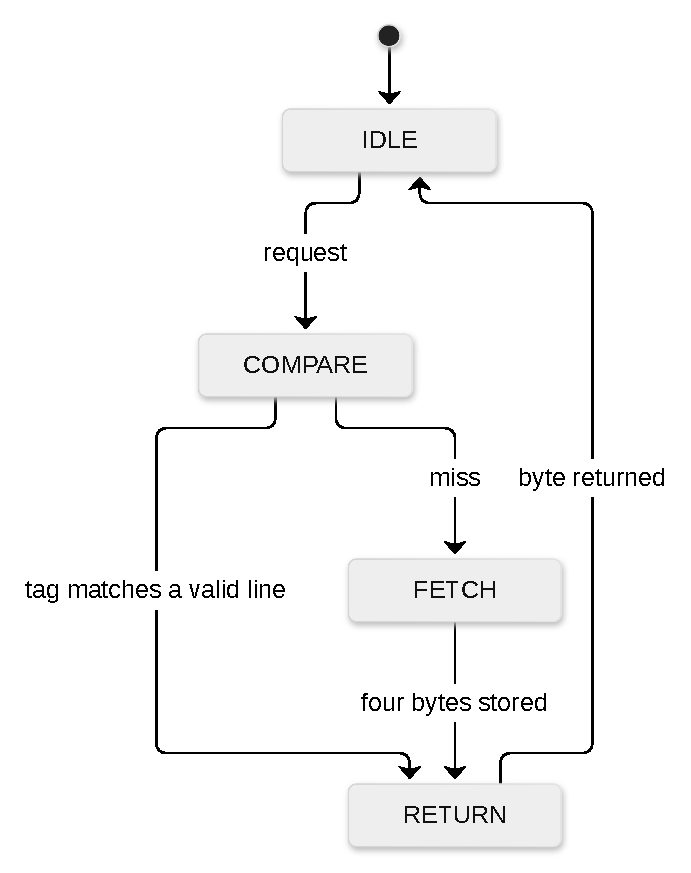
\includegraphics[height=0.28\textheight,keepaspectratio]{states.pdf}
\caption{LRU controller. A hit does not enter \texttt{FETCH}. Diagram drawn with Mermaid~\cite{mermaid}.}
\label{fig:states}
\end{figure}

The fill reuses the same one-line fetch sequence as the board design: four reads, then a single-cycle done. A new fill request is ignored on the cycle \texttt{fetch\_done} is still high, so one miss cannot start a second fill. The byte order inside a line is fixed. Offset~0 is the least significant byte of the fetched word, which is the byte at the block base. Offset~3 is the last byte of the line.

\chapter{Exhaustive checks of the LRU cache}
\label{ch:tests}

The testbench drives the LRU register-transfer design and checks every access three ways. The returned byte equals the address. Hit and miss are mutually exclusive. A miss has \texttt{mem\_read} high on some cycle before done, and a hit never does. The simulator is Icarus Verilog~12.0. The run reported \texttt{ALL TESTS PASSED}.

\begin{table}[ht]
\centering
\caption{LRU accesses in one simulation run. The cache is cleared at the start of each temporal block, each spatial start, and each later scenario.}
\label{tab:counts}
\begin{tabular}{lrrr}
\toprule
Check & Accesses & Hits & Misses \\
\midrule
Temporal, 64 blocks \(\times\) 5 reads & 320 & 256 & 64 \\
Spatial, 64 blocks \(\times\) 4 starts \(\times\) 4 bytes & 1024 & 768 & 256 \\
Empty line, \texttt{0x00} then \texttt{0x10} & 4 & 2 & 2 \\
Victim rotation, four choices & 52 & 28 & 24 \\
Capacity walk, blocks 0 to 63 & 69 & 4 & 65 \\
Comparison sequences in \cref{ch:compare} & 29 & 18 & 11 \\
\midrule
Total & 1498 & 1076 & 422 \\
\bottomrule
\end{tabular}
\end{table}

All \num{422} misses read memory. None of the \num{1076} hits did. No access timed out, and no access returned a byte other than its address.

\section{Temporal locality}

For each of the 64 blocks the cache is cleared and the block base is read five times. The first read misses and fills the line. The next four hit, and memory stays idle. That is temporal locality: the same address, again, is answered from the line just installed~\cite{patterson2021}. Five reads on 64 blocks give the 64~misses and 256~hits in \cref{tab:counts}.

\section{Spatial locality}

For each block, and for each of the four bytes as the first request, the cache is cleared and that byte is read, then the other three bytes of the same line. The first byte misses. The other three hit, including the case that walks off the end of the line and wraps to offset~0, because a fill always stores the whole aligned line. The neighbouring bytes were not requested, and they are present anyway. That is spatial locality. The 256~first bytes account for every spatial miss. The 768~followers are hits.

\section{An empty line is used before a resident line}

After a reset, \texttt{0x00} misses into line~0 and \texttt{0x10} misses into line~1. Both addresses then hit. The second block did not overwrite the first. Three lines were still empty, so there was no reason to evict.

\section{The untouched line is the one replaced}

Four blocks, \texttt{0x00}, \texttt{0x04}, \texttt{0x08} and \texttt{0x0C}, fill the cache and leave the ages in \cref{tab:ages}. The test then reads every block except one. Those three hit, and the skipped block becomes the unique least recently used line. The new block \texttt{0x10} misses and must take that line.

The three survivors and \texttt{0x10} are read back before the displaced address is read again. They hit. The displaced address misses. Doing it in that order matters: reading the displaced address is itself a miss, and that miss would replace one of the survivors if it were issued first. The four choices of which block to skip all passed. In each case the block that was left untouched was the block \texttt{0x10} replaced.

\section{Capacity}
\label{sec:capacity}

The cache is filled by reading every block base from \texttt{0x00} through \texttt{0xFC}, 64~misses. Only four lines exist, so each new block after the fourth replaces the oldest resident block. At the end the resident blocks are \texttt{0xF0}, \texttt{0xF4}, \texttt{0xF8} and \texttt{0xFC}. Those four hit. Block \texttt{0xEC}, which was resident earlier and was then pushed out, misses. The four hits are taken before that miss, because the miss would itself replace the oldest of the four.

A shorter capacity check is in the comparison. The four lines \texttt{0x00}, \texttt{0x04}, \texttt{0x08} and \texttt{0x0C} miss on the way in and hit on the way round again. The working set fits, so the repeat is all hits. The same eight decisions appear in the direct-mapped column, because those four addresses use four different indices.

\chapter{Where the two policies differ}
\label{ch:compare}

The comparison uses five address lists. Each list is applied to the LRU design, and the same list is scored with the direct-mapped rule: index \texttt{address[3:2]}, tag \texttt{address[7:4]}, valid bit, one line per index. That rule is the one already measured on the board. This column is that rule, stepped in lockstep with the LRU simulation. It is the placement function, recorded beside the new design.

\begin{table}[ht]
\centering
\caption{Hit and miss on the same addresses. H is a hit, M is a miss. The cache starts empty for each row.}
\label{tab:compare}
\begin{tabular}{lll}
\toprule
Sequence & Direct-mapped & LRU \\
\midrule
Temporal \texttt{0x00} five times & MHHHH & MHHHH \\
Spatial \texttt{0x00}--\texttt{0x07} & MHHH MHHH & MHHH MHHH \\
Conflict \texttt{0x00}, \texttt{0x10}, \texttt{0x00}, \texttt{0x10} & MMMM & MMHH \\
Capacity \texttt{0x00}, \texttt{0x04}, \texttt{0x08}, \texttt{0x0C}, twice & MMMM HHHH & MMMM HHHH \\
Replacement \texttt{0x00}, \texttt{0x00}, \texttt{0x10}, \texttt{0x00} & MHMM & MHMH \\
\bottomrule
\end{tabular}
\end{table}

\section{Locality does not separate them}

The temporal row is one address. The first reference misses in both caches and fills one line. The next four references match that line. Nothing is ever evicted, so the replacement policy is idle.

The spatial row crosses one block boundary. \texttt{0x00} fills the line that also holds \texttt{0x01}, \texttt{0x02} and \texttt{0x03}. \texttt{0x04} is the next line and misses. \texttt{0x05} to \texttt{0x07} hit from that second fill. Direct mapping and full associativity store a spatial line the same way. The traces match, as \cref{tab:compare} shows. Locality explains why a line is worth filling. It does not explain why one placement rule beats the other.

\section{Conflict}

\texttt{0x00} and \texttt{0x10} share index~0, so the direct-mapped cache has only one place for either of them. Each of the four references misses, and each miss reads memory. The shapes are in \cref{fig:conflict-dm}. The LRU cache has a free line for \texttt{0x10}. The third and fourth references hit, and memory stays idle, as in \cref{fig:conflict-lru}. Both blocks still fit. The misses that remain in the direct-mapped trace are conflict misses~\cite{hill1989}.

\begin{figure}[H]
\centering
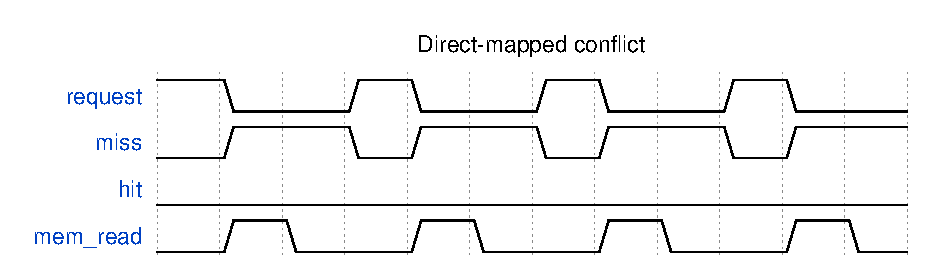
\includegraphics[width=0.92\textwidth]{conflict-dm.pdf}
\caption{Direct-mapped conflict on \texttt{0x00}, \texttt{0x10}, \texttt{0x00}, \texttt{0x10}. Every reference misses and reads memory. The drawing is the decision shape, compressed so the labels stay readable. WaveDrom~\cite{wavedrom}.}
\label{fig:conflict-dm}
\end{figure}

\begin{figure}[H]
\centering
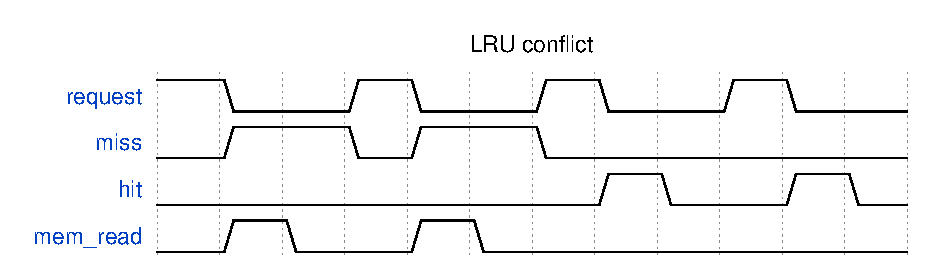
\includegraphics[width=0.92\textwidth]{conflict-lru.pdf}
\caption{The same four addresses on the LRU cache. The first visit to each block misses. The second visit hits, because the two blocks occupy two lines.}
\label{fig:conflict-lru}
\end{figure}

\section{Replacement}

The replacement list is \texttt{0x00}, again \texttt{0x00}, then \texttt{0x10}, then \texttt{0x00}. Both caches miss, hit, miss on the first three references. The fourth is the point. In the direct-mapped cache, \texttt{0x10} occupies the only line \texttt{0x00} can use, so the last reference misses and reads memory (\cref{fig:replace-dm}). In the LRU cache, \texttt{0x10} took an empty line and the age update left \texttt{0x00} resident, so the last reference hits (\cref{fig:replace-lru}).

\begin{figure}[H]
\centering
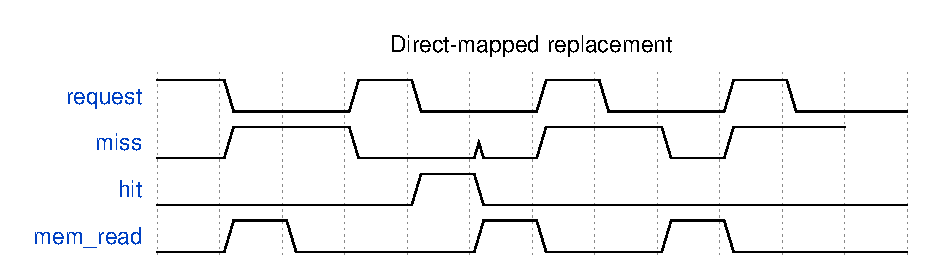
\includegraphics[width=0.92\textwidth]{replace-dm.pdf}
\caption{Direct-mapped replacement. After \texttt{0x10} takes line~0, the return to \texttt{0x00} misses.}
\label{fig:replace-dm}
\end{figure}

\begin{figure}[H]
\centering
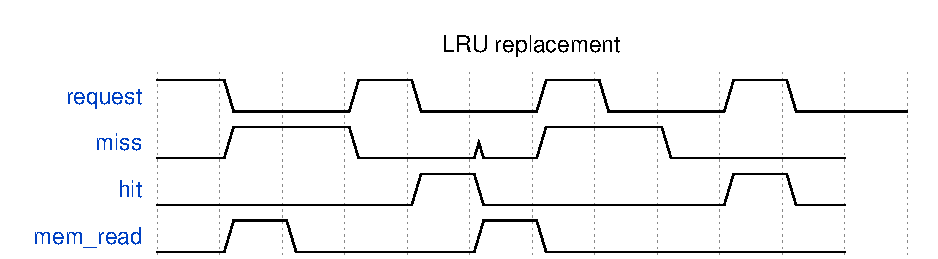
\includegraphics[width=0.92\textwidth]{replace-lru.pdf}
\caption{LRU replacement of the same addresses. \texttt{0x10} does not remove \texttt{0x00}, so the last reference hits.}
\label{fig:replace-lru}
\end{figure}

\section{What the comparison is for}

Temporal and spatial rows are the control. They should match, and they do. Conflict and replacement are the measurement. Same capacity, same addresses, different traces, and the difference is exactly the line that direct mapping was forced to overwrite. Capacity matches on the four-line working set because that set fits in both organisations. The long walk in \cref{sec:capacity} is an LRU-only check of which four blocks survive a pass through the whole memory.

\chapter{Limit of the claim}
\label{ch:limit}

The LRU result is a simulation of the register-transfer design: \num{1498} accesses, the byte check, the exclusive hit or miss, and the memory-read rule, all passing. The direct-mapped column is the index and tag rule of the cache that has already been run on the Shrike Lite. This report does not add a second bitstream, and it does not claim that the LRU cache has been observed on the logic analyser.

On the Horizon~2020 scale the direct-mapped board design remains the laboratory validation~\cite{ectrl}. The LRU cache is a proof of the placement function under an exhaustive read-only stimulus. That is short of laboratory validation. Writes, a processor, and a real program are outside both designs. The bibliography file can be imported into Zotero; the citations here are numeric and were compiled with BibLaTeX.

\chapter{Conclusion}

A fully associative LRU cache of four lines, simulated on its own, answers the question the direct-mapped board left open. Repeated references and the other bytes of a filled line behave the same under both rules. Two blocks that share an index do not. Direct mapping misses on every visit to \texttt{0x00} and \texttt{0x10}. The LRU cache misses once each and then hits, and it still holds \texttt{0x00} after \texttt{0x10} has been installed. The untouched line is the line a new block replaces. Those are the traces worth having. A larger cache would have hidden them.

\printbibliography[heading=bibintoc]

\end{document}
